\documentclass[12pt, a4paper]{article}

\usepackage[utf8]{vietnam}
\usepackage{graphicx}
\usepackage{booktabs}
\usepackage{hyperref}
\usepackage{amsmath,amssymb}
\usepackage{enumitem}
\usepackage[top=2cm, bottom=2cm, left=2.5cm, right=2cm]{geometry}
\graphicspath{{images/}}

\begin{document}

\begin{center}
    {\Large \textbf{BÁO CÁO BÀI TẬP TUẦN 4}}\\[0.3em]
    {\large Mã hóa Sequential Counter cho ràng buộc thứ tự (B3)}
\end{center}

\section{Mục tiêu và phương pháp}
Tuần 4 tập trung vào ràng buộc \textbf{Precedence} (thứ tự đi đường của một tàu trên hai ga liên tiếp $r \prec_i q$), tạm gọi là B3: nếu tàu $i$ xuất phát ở ga $r$ tại thời điểm $h_{ir}^{p}$ thì nó chỉ được xuất phát ở ga $q$ sau $h_{ir}^{p} + l_r$ (với $l_r$ là thời gian chiếm dụng tối thiểu ga $r$). Theo hướng dẫn, mục tiêu là xây dựng mã hóa \textbf{Sequential Counter} trên biến tích lũy $R_{iq,1,t}$.

Các file trong thư mục \texttt{submissions/tuan4\_doquangvinh/}:
\begin{itemize}
    \item \texttt{bai1\_scl\_precedence.py} - mã hóa SCL (C1-C7), mã hóa Direct baseline và ràng buộc Exactly-One;
    \item \texttt{bai2\_bruteforce\_checker.py} - bộ duyệt vét cạn kiểm chứng tính tương đương nghiệm giữa Direct và Sequential Counter;
    \item \texttt{run\_experiments\_week4.py} - benchmark 12 cấu hình và vẽ 3 biểu đồ chỉ tiêu;
    \item \texttt{experiment\_results.csv}, \texttt{images/*.png} - số liệu và trực quan hóa.
\end{itemize}

\section{Mã hóa Sequential Counter for Ladder cho ràng buộc thứ tự (Bài 1)}
Ý tưởng cốt lõi: thay vì sinh mệnh đề cho từng cặp interval $(x_{ir}^p, x_{iq}^t)$ như Direct (bùng nổ $O(n \times m)$), ta đưa vào $m$ biến tích lũy $R_{iq, 1, t}$ với ý nghĩa
$$
    R_{iq, 1, t} = 1 \Leftrightarrow \text{tàu đã xuất phát ở ga } q \text{ tại interval } \le t .
$$
Nhờ đó mỗi interval $p$ của ga $r$ chỉ cần $1$ mệnh đề: nếu $r$ xuất phát tại thời điểm $h_{ir}^p$ thì $q$ phải bắt đầu sau $h_{ir}^p + l_r$, tức $\neg R_{K_p}$ với $K_p = \max\{t \mid h_{iq}^t < h_{ir}^p + l_r\}$. Bộ mệnh đề đầy đủ (C1-C7):
\begin{itemize}
    \item (C1) $R_1 \rightarrow x^q_1$ và (C2) $x^q_1 \rightarrow R_1$ - base case;
    \item với $t = 2 \dots m$: (C2) $x_{iq}^t \rightarrow R_{iq, 1, t}$; (C3) $R_{iq, 1, t-1} \rightarrow R_{iq, 1, t}$ (tính đơn điệu của biến tích lũy); (C4) $R_{iq, 1, t} \rightarrow R_{iq, 1, t-1} \lor x_{iq}^t$; (C5) $R_{iq, 1, t-1} \rightarrow \neg x_{iq}^t$;
    \item (C6) $R_{iq, 1, m}$ (đơn nguyên - ép tàu chắc chắn phải xuất phát ở ga $q$);
    \item (C7) $x_{ir}^{p} \rightarrow \neg R_{iq, 1, K_p}$ (rút gọn biên: nếu $K_p = 0$ bỏ qua, $K_p = m$ cấm hẳn $x^r_p$).
\end{itemize}
Số mệnh đề sinh ra đúng bằng $4m - 1 + n$ và số biến $= (n + m) + m$ (thêm $m$ biến $R$), tức \textbf{tuyến tính} $O(n + m)$, so với $O(n \times m)$ của mã hóa trực tiếp vì Direct phải xét mọi cặp quá sớm.

\section{Kiểm chứng tính tương đương nghiệm bằng brute-force (Bài 2)}
Script \texttt{bai2\_bruteforce\_checker.py} kiểm chứng: \emph{công thức CNF (SCL + Exactly-One) có diễn đạt đúng ràng buộc vật lý không}:
\begin{enumerate}[label = (\roman*)]
    \item \texttt{physical\_b3\_ok} - định nghĩa nghiệm vật lý: Exactly-One trên $x_{iq}$ + precedence B3;
    \item \texttt{cnf\_satisfied} với Direct + Exactly-One;
    \item \texttt{cnf\_satisfied} với SCL + Exactly-One khi có gán biến $R$.
\end{enumerate}
Với mỗi gán biến quyết định (duyệt đủ $2^{n+m}$ tổ hợp bằng bitmask), chương trình xét thêm $2^m$ tổ hợp cho biến phụ $R$. Mismatch chỉ xảy ra khi kết quả của hai mã hóa CNF khác với kết quả vật lý. Chạy ở bốn giá trị biên $l_r \in \{0, 5, 15, 100\}$ (góc 0, khoảng giữa, biên, lớn hơn mọi interval), mọi phép gán đều cho \textbf{0 mismatch}. Kết luận: cả Direct lẫn SCL đều tương đương nghiệm 100\% với B3 + Exactly-One.

Hai điểm phát hiện trong quá trình kiểm thử đã được khắc phục trước khi hoàn thành:
\begin{itemize}
    \item Phải cộng \textbf{Exactly-One} vào cả Direct lẫn SCL để cả hai thao tác trên cùng tiền đề B1; nếu chỉ SCL có EO, các gán vi phạm B1 sẽ khiến Direct ``chấp nhận oan'' và gây mismatch giả;
    \item SCL cần thêm chiều ngược của (C1), tức $R_1 \rightarrow x^q_1$, để $R_1$ không bao giờ nhận giá trị 1 khi tàu chưa xuất phát - bảo toàn nghĩa tích lũy.
\end{itemize}

\section{Kết quả thực nghiệm}
Dùng \texttt{run\_experiments\_week4.py} quét 12 cấu hình với $m \in \{8,16,32,64\}$, $n \in \{4,8,16\}$ và đo chỉ tiêu bằng solver CaDiCaL153 qua PySAT (số liệu đầy đủ trong \texttt{experiment\_results.csv}). Do chọn $l_r = 5 \times m$, mỗi interval $p$ ở ga $r$ chặn khoảng $\frac{m}{2}$ interval ở ga $q$: Direct phải sinh một mệnh đề cho từng cặp trong khối đó (bùng nổ bậc hai), còn SCL chỉ tốn một mệnh đề mỗi $p$ cộng chuỗi tuyến tính $R$.

Bảng dưới tóm tắt số mệnh đề và số biến theo $m$ (với $n = 16$ cố định):
\begin{table}[htbp]
    \centering
    \small
    \caption{Số mệnh đề và số biến khi $n = 16$, $l_r = 5 \cdot m$.}
    \label{tab:clauses}
    \begin{tabular}{lrrrr}
        \toprule
        $m$ & Direct (clauses) & SCL (clauses) & Direct (vars) & SCL (vars)\\
        \midrule
        8  & 118 & 47  & 24 & 32\\
        16 & 220 & 79  & 32 & 48\\
        32 & 376 & 143 & 47 & 80\\
        64 & 632 & 271 & 63 & 144\\
        \bottomrule
    \end{tabular}
\end{table}

Hình \ref{fig:clauses} và \ref{fig:variables} cho thấy xu hướng rõ rệt: khi $m$ tăng, số mệnh đề Direct tăng nhanh (bậc hai theo $n \times m$), còn SCL chỉ tăng \emph{tuyến tính} theo $4m$ và gần như \emph{không đổi theo $n$}. Đây chính là lợi thế quyết định của SCL khi số interval $m$ và số ga $n$ lớn.

\begin{figure}[htbp]
    \centering
    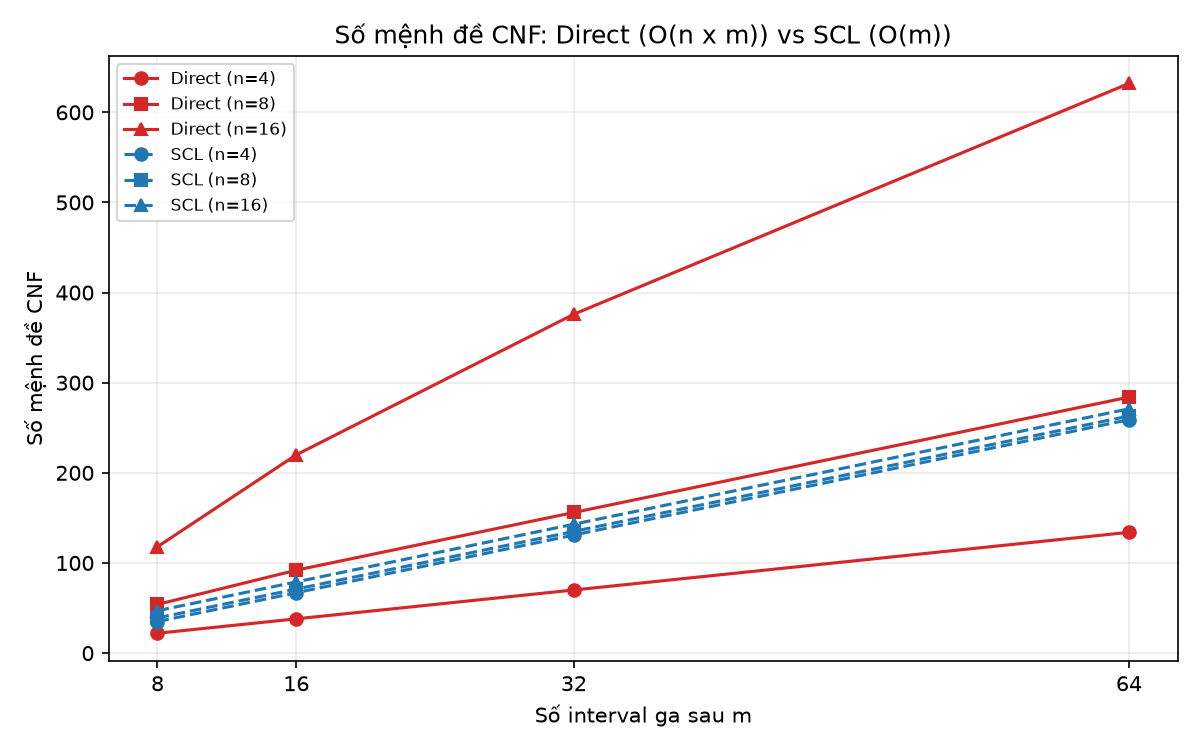
\includegraphics[width=0.9\textwidth]{cnf_clauses_comparison.png}
    \caption{Số mệnh đề: Direct $O(n\times m)$ vs SCL $O(n+m)$.}
    \label{fig:clauses}
\end{figure}

\begin{figure}[htbp]
    \centering
    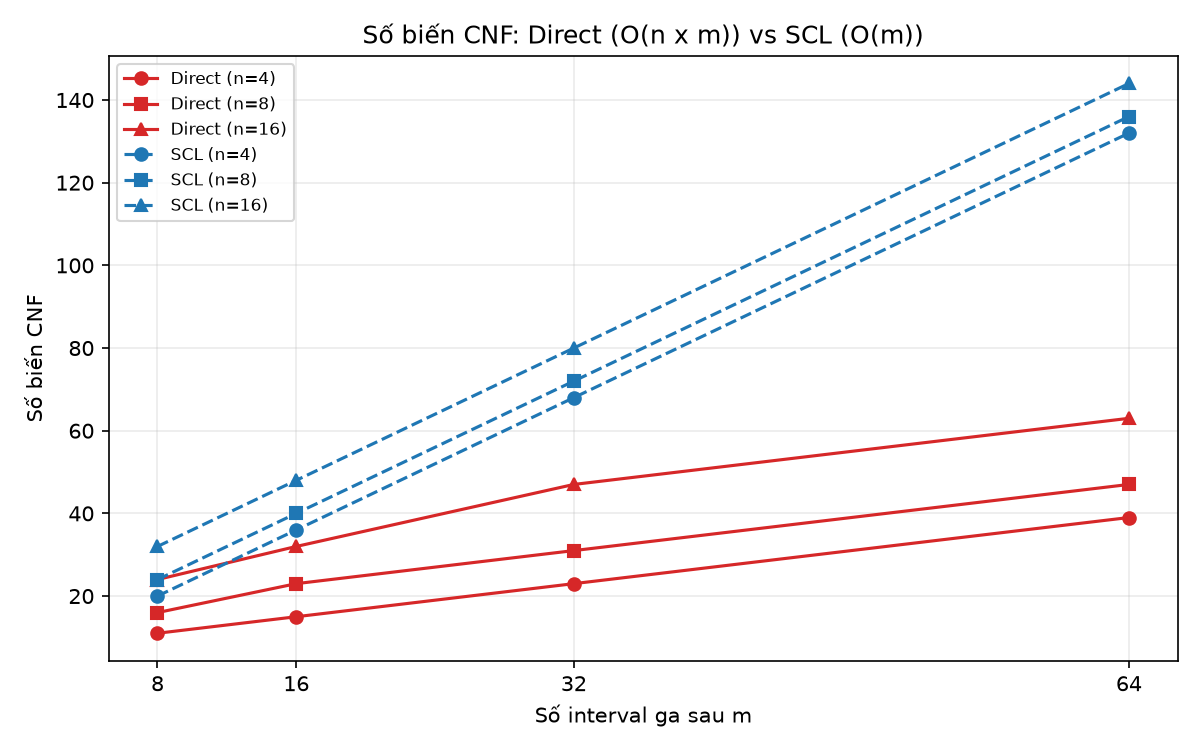
\includegraphics[width=0.9\textwidth]{cnf_variables_comparison.png}
    \caption{Số biến: SCL đổi thêm $m$ biến $R$ để giảm số mệnh đề.}
    \label{fig:variables}
\end{figure}

\section{Kết luận}
Tuần 4 đã mã hóa ràng buộc thứ tự B3 bằng SCL (C1-C7) với biến tích lũy $R$, đạt số mệnh đề tuyến tính $4m - 1 + n$ thay vì bậc hai như Direct. Bộ brute-force xác nhận công thức tương đương 100\% với ràng buộc vật lý B3 + Exactly-One trên toàn bộ không gian gán (duyệt $2^{n+m}$ gán $\times$ $2^m$ gán $R$). Thực nghiệm với CaDiCaL153 khẳng định SCL tăng tuyến tính trong khi Direct tăng bậc hai, chứng tỏ phương pháp đáng dùng khi $m$ và $n$ lớn.

\section{Sản phẩm}
\begin{itemize}
    \item \textbf{Bài 1}: \texttt{bai1\_scl\_precedence.py} - mã hóa SCL (C1--C7), Direct, Exactly-One.
    \item \textbf{Bài 2}: \texttt{bai2\_bruteforce\_checker.py} - kiểm chứng tương quy logic.
    \item \textbf{Bài 3}: \texttt{run\_experiments\_week4.py} + \texttt{experiment\_results.csv} + 3 biểu đồ trong \texttt{images/}.
    \item \textbf{Báo cáo}: \texttt{bao\_cao\_tuan\_4.tex}.
    \item \textbf{Repository Git}: \url{https://github.com/Viing3107/maxsattrainscheduling/tree/tuan4_doquangvinh}
\end{itemize}

\end{document}